%\documentstyle[epsf,twocolumn]{jarticle}       %LaTeX2.09仕様
\documentclass[twocolumn]{jarticle}     %pLaTeX2e仕様

%\usepackage[backend=bibtex, style=numeric]{biblatex}
%\addbibresource{sankou.bib}
%%%%%%%%%%%%%%%%%%%%%%%%%%%%%%%%%%%%%%%%%%%%%%%%%%%%%%%%%%%%%%
%%
%%  基本 バージョン
%%
%%%%%%%%%%%%%%%%%%%%%%%%%%%%%%%%%%%%%%%%%%%%%%%%%%%%%%%%%%%%%%%%
\setlength{\topmargin}{-45pt}
%\setlength{\oddsidemargin}{0cm}
\setlength{\oddsidemargin}{-7.5mm}
%\setlength{\evensidemargin}{0cm}
\setlength{\textheight}{24.1cm}
%setlength{\textheight}{25cm}
\setlength{\textwidth}{17.4cm}
%\setlength{\textwidth}{172mm}
\setlength{\columnsep}{11mm}

\setlength{\intextsep}{8pt}
\setlength{\textfloatsep}{8pt}
\setlength{\floatsep}{1pt}

\kanjiskip=.07zw plus.5pt minus.5pt



%【節がかわるごとに(1.1)(1.2) …(2.1)(2.2)と数式番号をつけるとき】
%\makeatletter
%\renewcommand{\theequation}{%
%\thesection.\arabic{equation}} %\@addtoreset{equation}{section}
%\makeatother

%\renewcommand{\arraystretch}{0.95} 行間の設定

\usepackage[dvipdfmx]{graphicx}   %pLaTeX2e仕様(\documentstyle ->\documentclass)
\usepackage[dvipdfmx]{color}
\usepackage{scalefnt}
\usepackage{bm}
\usepackage{here}
\usepackage{url}
\usepackage{amsmath}
\usepackage{amsfonts}
\usepackage[subrefformat=parens]{subcaption}
\captionsetup{compatibility=false}
%%%%%%%%%%%%%%%%%%%%%%%%%%%%%%%%%%%%%%%%%%%%%%%%%%%%%%%%
\usepackage{comment}
\usepackage{subcaption}
\usepackage{multirow}
\usepackage{nidanfloat}
%\usepackage[table,xcdraw]{xcolor}
\usepackage[dvipdfmx]{hyperref}

\usepackage[normalem]{ulem}
\useunder{\uline}{\ul}{}

\begin{document}

\twocolumn[
\noindent
\hspace{1em}

令和2年6月17日(水) ゼミ資料
\hfill
\ \ B4 高山 裕成

\vspace{2mm}
\hrule
\begin{center}
{\Large  進捗報告}
\end{center}
\hrule
\vspace{3mm}
]

\section{あらすじ}
サブワード化しよう.

% \footnotesize
\section{進捗}

\begin{itemize}
  \item サブワード化したデータでの正例ラベルを喜楽・ニュートラル・驚愕としたときの 2 クラス感情推定
\end{itemize}

\section{実験設定}
BERT のトークナイザーを用いてサブワード化したデータを用いて, 最終レイヤーのみのチューニング (BERT Last Layer), またはすべてのパラメータを固定させる (BERT Fixed) 条件で BERT fine-tuning を追加で行った. 正例ラベルとして喜楽・ニュートラル・驚愕の 3 パターンについて 2 クラス分類を行った. 識別器としては 3 層 MLP を用いた.

MLP のパラメータを図\ref{table:net_para} に, 学習パラメータを表\ref{table:ex_para} に示す. 学習率は optuna によって最適化されたものを用いた. (試行回数 5 回)

先週, 意見としてあった, `!', `?' をトークンに置き換えることはせず, また入力 id 列の長さはサブワード化した時の最大系列長に合わせており, 固定サイズ (64, 128, ...) にはしていない.

\begin{table}[htb]
\caption{MLP パラメータ}
\label{table:net_para}
\centering
\begin{tabular}{|c||c|}
\hline
& MLP \\ \hline
(in,hidden,out) & (300,30,2)\\ \hline
dropout rate & 0.5 \\ \hline
activation function & tanh\\ \hline
\end{tabular}
\end{table}

\begin{table}[htb]
\caption{学習パラメータ}
\label{table:ex_para}
\centering
\begin{tabular}{|c||c|c|}
\hline
& \multicolumn{2}{|c|}{実験} \\ \hline
epoch & \multicolumn{2}{|c|}{200}  \\ \hline
batch size & \multicolumn{2}{|c|}{16} \\ \hline
loss function & \multicolumn{2}{|c|}{Cross Entropy Loss} \\ \hline
optimizer & \multicolumn{2}{|c|}{Adam} \\ \hline
\end{tabular}
\end{table}

\section{実験結果}
表\ref{tab:result} に実験結果を載せる. 比較対象として前回までの実験結果も載せている. 表\ref{tab:result} よりサブワード化しない場合と比べて, 指定した正例ラベルによっては精度の改善が若干見られたが全体的な優位性は見られなかった.

\section{問題点}
\begin{itemize}
  \item train と validation のデータ分布が似ているため, 場合によっては validation の accuracy が 1 になっていたりする.
  \item 実験中 Connection reset by 192.168.0.11 port 22 が出た.
\end{itemize}

\begin{table*}[!b]
\begin{center}
\caption{result}
\scalebox{0.5}{
\begin{tabular}{llllllllllllllllll|lll}
  \hline
   & \multicolumn{2}{c}{\multirow{2}{*}{model}} & \multicolumn{3}{c}{ギャグ} & \multicolumn{3}{c}{少女漫画} & \multicolumn{3}{c}{少年漫画} & \multicolumn{3}{c}{青年漫画} & \multicolumn{3}{c|}{萌え系} & \multicolumn{3}{c|}{5タッチ平均} \\
   & \multicolumn{2}{c}{} & \multicolumn{1}{c}{Acc} & \multicolumn{1}{c}{Recall} & \multicolumn{1}{c}{F1} & \multicolumn{1}{c}{Acc} & \multicolumn{1}{c}{Recall} & \multicolumn{1}{c}{F1} & \multicolumn{1}{c}{Acc} & \multicolumn{1}{c}{Recall} & \multicolumn{1}{c}{F1} & \multicolumn{1}{c}{Acc} & \multicolumn{1}{c}{Recall} & \multicolumn{1}{c}{F1} & \multicolumn{1}{c}{Acc} & \multicolumn{1}{c}{Recall} & \multicolumn{1}{c|}{F1} & \multicolumn{1}{c}{Acc} & \multicolumn{1}{c}{Recall} & \multicolumn{1}{c}{F1} \\ \hline
  \multirow{4}{*}{Juman++} & 驚愕 & BERT (Last Layer) & 0.758 & 0.000 & 0.000 & 0.806 & 0.000 & 0.000 & 0.859 & 0.000 & 0.000 & 0.662 & 0.647 & 0.500 & 0.719 & 0.000 & 0.000 & 0.761 & 0.129 & {\ul 0.100} \\ \cline{2-21}
   & ニュートラル & BERT (Last Layer) & 0.379 & 0.400 & 0.281 & 0.881 & 0.000 & 0.000 & 0.578 & 0.788 & 0.658 & 0.677 & 0.200 & 0.276 & 0.625 & 0.267 & 0.250 & 0.628 & 0.331 & {\ul 0.293} \\ \cline{2-21}
   & \multirow{2}{*}{喜楽} & BERT (Last Layer) & 0.833 & 0.400 & 0.421 & 0.567 & 0.579 & 0.603 & 0.797 & 0.083 & 0.133 & 0.800 & 0.357 & 0.435 & 0.656 & 0.455 & 0.476 & 0.731 & 0.375 & {\ul 0.414} \\
   &  & BERT (Fixed) & 0.818 & 0.500 & 0.455 & 0.463 & 0.421 & 0.471 & 0.766 & 0.000 & 0.000 & 0.769 & 0.429 & 0.444 & 0.625 & 0.409 & 0.429 & 0.688 & 0.352 & 0.360 \\ \hline
  \multirow{6}{*}{Subword} & \multirow{2}{*}{驚愕} & BERT (Last Layer) & 0.803 & 0.000 & 0.000 & 0.866 & 0.000 & 0.000 & 0.875 & 0.222 & 0.333 & 0.739 & 0.235 & 0.320 & 0.734 & 0.000 & 0.000 & 0.803 & 0.091 & 0.131 \\
   &  & BERT (Fixed) & 0.758 & 0.000 & 0.000 & 0.836 & 0.000 & 0.000 & 0.875 & 0.444 & 0.500 & 0.677 & 0.353 & 0.364 & 0.750 & 0.167 & 0.200 & 0.779 & 0.193 & {\ul 0.213} \\ \cline{2-21}
   & \multirow{2}{*}{ニュートラル} & BERT (Last Layer) & 0.561 & 0.650 & 0.473 & 0.896 & 0.000 & 0.000 & 0.516 & 0.727 & 0.608 & 0.662 & 0.200 & 0.267 & 0.729 & 0.333 & 0.357 & 0.672 & 0.382 & {\ul 0.341} \\
   &  & BERT (Fixed) & 0.485 & 0.450 & 0.346 & 0.910 & 0.000 & 0.000 & 0.563 & 0.697 & 0.622 & 0.631 & 0.250 & 0.294 & 0.703 & 0.200 & 0.240 & 0.658 & 0.319 & 0.300 \\ \cline{2-21}
   & \multirow{2}{*}{喜楽} & BERT (Last Layer) & 0.818 & 0.200 & 0.250 & 0.627 & 0.737 & 0.691 & 0.734 & 0.000 & 0.000 & 0.754 & 0.500 & 0.467 & 0.563 & 0.273 & 0.300 & 0.699 & 0.342 & 0.342 \\
   &  & BERT (Fixed) & 0.758 & 0.200 & 0.200 & 0.552 & 0.684 & 0.634 & 0.797 & 0.000 & 0.000 & 0.785 & 0.357 & 0.417 & 0.719 & 0.455 & 0.526 & 0.722 & 0.339 & {\ul 0.355} \\ \hline
   & ベースライン &  & \multicolumn{1}{c}{0.85} & \multicolumn{1}{c}{0} & \multicolumn{1}{c}{0} & \multicolumn{1}{c}{0.43} & \multicolumn{1}{c}{0} & \multicolumn{1}{c}{0} & \multicolumn{1}{c}{0.81} & \multicolumn{1}{c}{0} & \multicolumn{1}{c}{0} & \multicolumn{1}{c}{0.78} & \multicolumn{1}{c}{0} & \multicolumn{1}{c}{0} & \multicolumn{1}{c}{0.66} & \multicolumn{1}{c}{0} & \multicolumn{1}{c|}{0} & \multicolumn{1}{c}{0.71} & \multicolumn{1}{c}{0} & \multicolumn{1}{c}{0}
\end{tabular}
\label{tab:result}
}
\end{center}
\end{table*}


\section{現状の 4 コマストーリーデータセットの加工}
図\ref{fig:dataset}に, 現状独自に加工してある 4 コマストーリーデータセット\cite{ueno_miki2018} の一部を示す.

\begin{figure*}[tbh]
  \begin{center}
    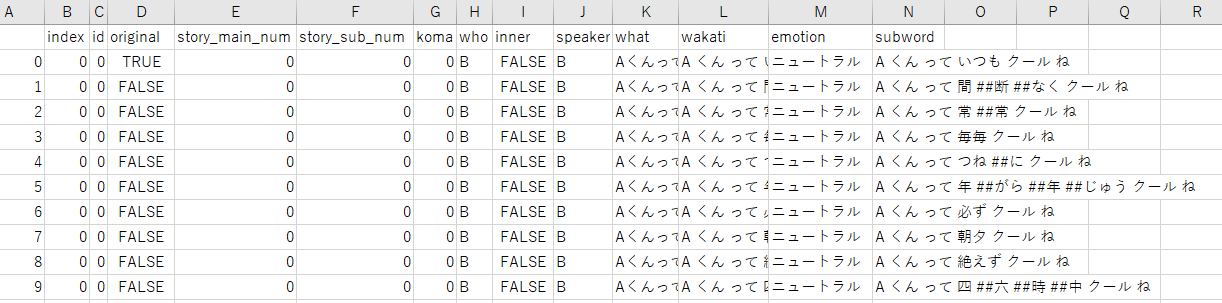
\includegraphics[scale=0.45]{dataset.png}
    \caption{dataset} %タイトルをつける
    \label{fig:dataset} %ラベルをつけ図の参照を可能にする
  \end{center}
\end{figure*}

\footnotesize
\begin{itemize}
  \item id : セリフの区別用の数字. 同じ id なら元は同じセリフから生成されている.
  \item original : オリジナルのセリフかどうか
  \item story main num : 第 n 話
  \item story sub num : 第 n 話の左右どちらか
  \item koma : 何コマ目に属するか
  \item who : 主体
  \item speaker : 話者
  \item inner : 傍白(主体にしか聞こえていないセリフ)かどうか
  \item what : セリフ
  \item wakati : what を juman++ で分かち書きにしたもの
  \item subword : wakati をさらに BERT のトークナイザーで分割したもの ([UNK] の場合は元の単語に戻している)
  \item emotion : 感情ラベル
\end{itemize}

\normalsize

\section{連続 n 文を入力とする実験のネットワークモデル}
図\ref{fig:net} にネットワークの概略図を示す. ${s_i}$ はそれぞれ連続する n 文のセリフを BERT の id 列に変換したものである. また, 組み合わせとしては同一の 4 コマに属し, かつ連続しているものを扱う. 各 4 コマの序盤に現れるセリフには参照できる過去のセリフが無いため, 便宜上のセリフ $[$pad$]$ を置くことで対処した. よって, 単語 id 列長を $w$ とすると入力次元は $(batch \times n \times w)$ となる. このままでは BERT の入力次元に対応していないので, まず $(n \times batch \times w)$ へと軸を入れ替え, これを 1 次元目について各要素に分解し, これら n 個の 次元数 $(batch \times w)$ のベクトルをそれぞれ BERT への入力とし, BERT の出力から [CLS] トークンに相当するベクトルのみを抜き取り, 先と逆の手順を踏むことで次元数 $(batch \times n \times 768)$ のテンソルを得ることができる. これを Bi LSTM, Self-Attention への入力とすることで末尾のセリフの感情推定を行う. このモデルの形で将来的に期待できることは, BERT の出力を stack する前に, 各 [CLS] Vector に元のセリフに対応するコマの画像の分散表現を concat でき, マルチモーダルでかつシーケンシャルな推定が可能となることであるが, 不安点としては BERT の利点を上手く利用できているのかという問題がある.

BERT は最終層のみをチューニングし, その他実験設定などは, 1 文のみを入力とする実験と同じである.

現状は, $n = 3$ として, テスト実験を回している. loss が下がっていることは確認できた.
計算時間は約 $3200 sec / 200 epoch$.

\begin{figure}[!hb]
  \begin{center}
    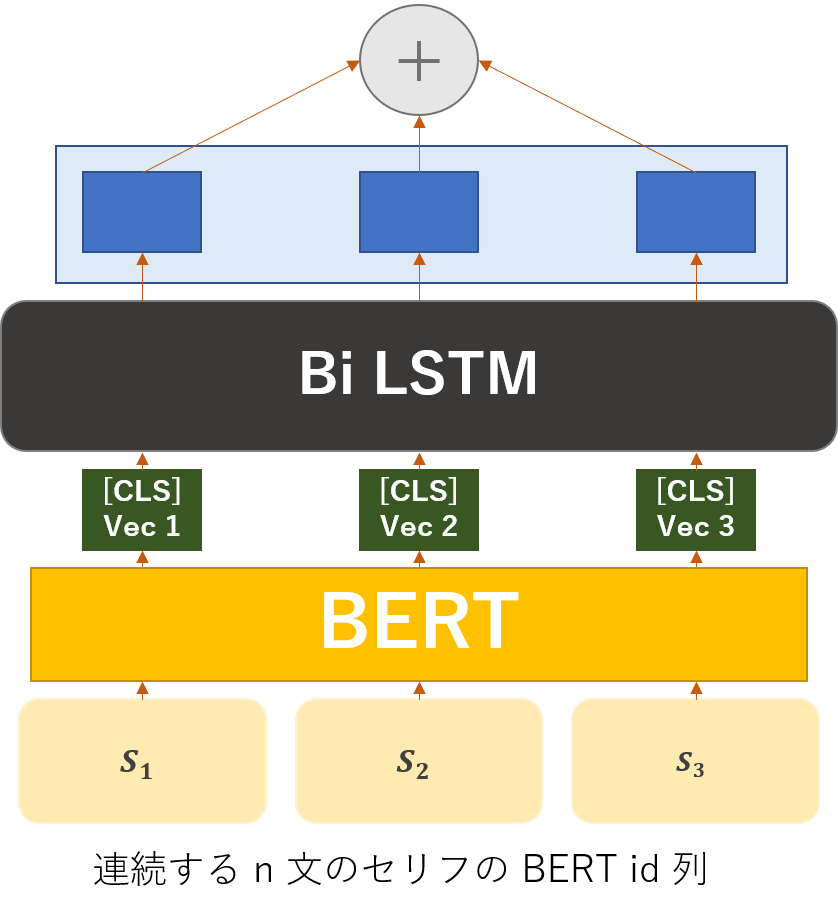
\includegraphics[scale=0.5]{net.png}
    \caption{seq net} %タイトルをつける
    \label{fig:net} %ラベルをつけ図の参照を可能にする
  \end{center}
\end{figure}

\newpage

\section{今後の実験予定}
\begin{itemize}
  \item 単語 id 列長を 64, 128 として実験
  \item 連続 n 文を入力とする実験
\end{itemize}

\bibliographystyle{unsrt}
\bibliography{sankou}


\end{document}
